\begin{pastexam}[label={px:gw3-104-ds-01}]{關務三等資訊處理 104 年 第一題}
（申論；20 分）

\[
C^{r}_{n} = \begin{cases} 0, & \text{若 } r > n \\ 1, & \text{若 } n == r \\ 1, & \text{若 } r == 0 \\
C^{n-1}_{r} + C^{n-1}_{r-1}, & \text{其他} \end{cases}
\quad\text{，兩項式係數的組合遞迴演算法公式如左。}
\]
\begin{itemize}[leftmargin=2.2em, nosep]
\item[㈠] 請用你熟悉的程式語言，撰寫此遞迴函式。（5 分）
\item[㈡] 若 $n$=5, $r$=3，請用二元樹畫出其遞迴呼叫的情形。（5 分）
\item[㈢] 最後的傳回值是多少？（5 分）
\item[㈣] 共遞迴呼叫幾次？（5 分）
\end{itemize}
\end{pastexam}

\begin{pastsoln}
答案：㈢ $10$。 ㈣ $19$ 次（含最外層那一次呼叫；只算遞迴產生的呼叫是 $18$ 次）。

原卷左邊寫 $C^{r}_{n}$（$n$ 在下、$r$ 在上），最後一行卻寫成
$C^{n-1}_{r} + C^{n-1}_{r-1}$，上下標對調了；照意思它是 $\binom{n-1}{r} + \binom{n-1}{r-1}$（巴斯卡公式），下面都寫成
$C(n, r)$。

\textbf{㈠} 照定義直接寫（C 語言）：
\begin{minted}[fontsize=\small]{c}
int C(int n, int r)
{
    if (r > n)
        return 0;
    if (n == r || r == 0)
        return 1;
    return C(n - 1, r) + C(n - 1, r - 1);
}
\end{minted}
從 $0 \le r \le n$ 開始呼叫時，$r > n$ 的情況其實不會出現：$n$ 減一時若 $r$ 不變，表示原本 $r < n$（$r = n$ 已經
在第二個 \texttt{if} 傳回），所以仍然 $r \le n - 1$。

\textbf{㈡ 遞迴樹。} 每個節點是一次呼叫 $C(n, r)$，左子節點是 $C(n-1, r)$、右子節點是 $C(n-1, r-1)$，葉子是直接傳回
$1$ 的呼叫；節點上的「$n,r$」表示呼叫 $C(n, r)$：
\begin{center}
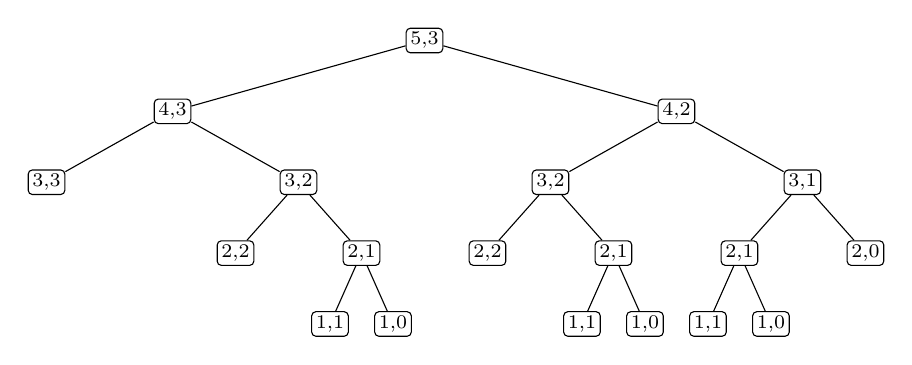
\begin{tikzpicture}[every node/.style={draw,rounded corners=1.5pt,inner sep=1.5pt,font=\scriptsize},
  level distance=9mm, level 1/.style={sibling distance=64mm}, level 2/.style={sibling distance=32mm},
  level 3/.style={sibling distance=16mm}, level 4/.style={sibling distance=8mm}]
\node {5,3}
  child {node {4,3}
    child {node {3,3}}
    child {node {3,2}
      child {node {2,2}}
      child {node {2,1} child {node {1,1}} child {node {1,0}}}}}
  child {node {4,2}
    child {node {3,2}
      child {node {2,2}}
      child {node {2,1} child {node {1,1}} child {node {1,0}}}}
    child {node {3,1}
      child {node {2,1} child {node {1,1}} child {node {1,0}}}
      child {node {2,0}}}};
\end{tikzpicture}
\end{center}

\textbf{㈢ 傳回值。} 由下往上：$C(2,1) = 1 + 1 = 2$，$C(3,2) = C(2,2) + C(2,1) = 3$，$C(3,1) = C(2,1) + C(2,0) = 3$，
$C(4,3) = 1 + 3 = 4$，$C(4,2) = 3 + 3 = 6$，$C(5,3) = 4 + 6 = 10$，就是 $\binom{5}{3} = 10$。

\textbf{㈣ 呼叫次數。} 數樹上的節點：$10$ 個葉子（每個葉子傳回 $1$，加起來正好是答案 $10$）、$9$ 個內部節點，共 $19$
個，也就是 $19$ 次呼叫。 一般而言 $C(n, r)$ 被呼叫 $2\binom{n}{r} - 1$ 次（資結書定理~18.1）：葉子有 $\binom{n}{r}$ 個，
每個內部節點恰有兩個子節點，內部節點比葉子少一個。 $2 \cdot 10 - 1 = 19$。 若「遞迴呼叫」只算函式呼叫自己的次數，
不算最外層的第一次，則是 $18$ 次。 上圖 $C(3,2)$、$C(2,1)$ 都被重複計算，用動態規劃（巴斯卡三角形）可以只算
$O(nr)$ 個值（資結書第~18.1~節）。
\end{pastsoln}
